\documentclass[a4paper]{article}
\usepackage{bookmark}
\usepackage{minted,xcolor}
\usepackage{graphicx}
\usepackage{hyperref}
\usepackage{geometry}
\usepackage{circuitikz}
\usepackage{tikz}
\usetikzlibrary{arrows,shapes,automata,petri,positioning,calc}
\usepackage{wrapfig}
\usepackage{caption}
\usepackage{subcaption}
\captionsetup{compatibility=false}
\usepackage{amsmath}
\usepackage{amssymb}
\usepackage[utf8]{inputenc}
\usepackage[export]{adjustbox}
\newcommand{\Sum} [2] {\the\numexpr #1 + #2 \relax \\}
\definecolor{mygray}{RGB}{238, 238, 238}
% \definecolor{bg}{RGB}{40,42,54}
\definecolor{bg}{RGB}{46, 46, 46}
\graphicspath{ {img/} }
\hypersetup{
    colorlinks=true,
    linkcolor=blue,
    filecolor=magenta,      
    urlcolor=orange,
}
\urlstyle{same}
\geometry{a4paper, margin=1in}
\usemintedstyle{monokai}
\title{ELP201 Lab Report 3}
\author{Adit Malhotra}
\date{2020EE10458}
\begin{document}
\maketitle
\tikzstyle{branch}=[fill,shape=circle,minimum size=2.5pt,inner sep=0pt]
\section{Introduction}
According to my entry number $(2020EE10458)$, the sequence to be generated at output side is $1,0,1,0,0,0$. 
\section{State diagram}
In total there would be 6 states, let them $S_{i}$, where $i \in \{0,1,2,3,4,5\}$. Let $S_{0}$ be the idle state. Then according to the statement of question the state diagram would be:
\begin{figure}[H]
  \centering
  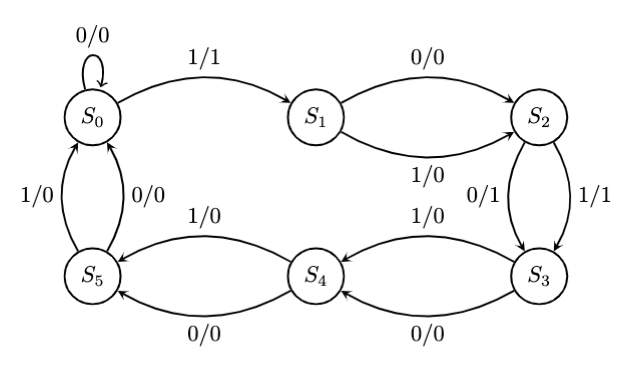
\includegraphics[width=0.7\textwidth]{states.png}
\end{figure}

Since total number of states are 6 and $6\leqslant 2^{3}$, hence total of 3 flipflops would be needed.\\
Let's assign each state $S_{i}$ the binary value of $i$.
\pagebreak
\section{State table}
The outputs $Q_{2}Q_{1}Q_{0}$, of the D-flipflops would represent the state at any time t. And since the characteristic equation for the D-flipflop is $Q(t+1) = D$, then the state table would be:
\begin{center}
	\begin{tabular}{||c c c || c || c c c|| c ||c c c||}
		\hline
		$Q_{2}(t)$ & $Q_{1}(t)$ & $Q_{0}(t)$ & $X (in)$ & $Q_{2}(t+1)$ & $Q_{1}(t+1)$ & $Q_{0}(t+1)$ & $Y (out)$ & $D_{2}$ & $D_{1}$ & $D_{0}$ \\ [0.5ex]
		\hline
		\hline
		0&0&0&0&0&0&0&0&0&0&0  \\ \hline
    0&0&0&1&0&0&1&1&0&0&1  \\ \hline
    0&0&1&0&0&1&0&0&0&1&0  \\ \hline
    0&0&1&1&0&1&0&0&0&1&0  \\ \hline
    0&1&0&0&0&1&1&1&0&1&1  \\ \hline
    0&1&0&1&0&1&1&1&0&1&1  \\ \hline
    0&1&1&0&1&0&0&0&1&0&0  \\ \hline
    0&1&1&1&1&0&0&0&1&0&0  \\ \hline
    1&0&0&0&1&0&1&0&1&0&1  \\ \hline
    1&0&0&1&1&0&1&0&1&0&1  \\ \hline
    1&0&1&0&0&0&0&0&0&0&0  \\ \hline
		1&0&1&1&0&0&0&0&0&0&0  \\ 
		\hline
	\end{tabular}
\end{center}
\section{Simplification using K-maps}
From the state table, the k-maps for $Output\  (Y),D_{2},D_{1},D_{0}$ are as follows:
\begin{figure}[H]
  \centering
  \begin{minipage}[c]{0.45\textwidth}
      \centering
      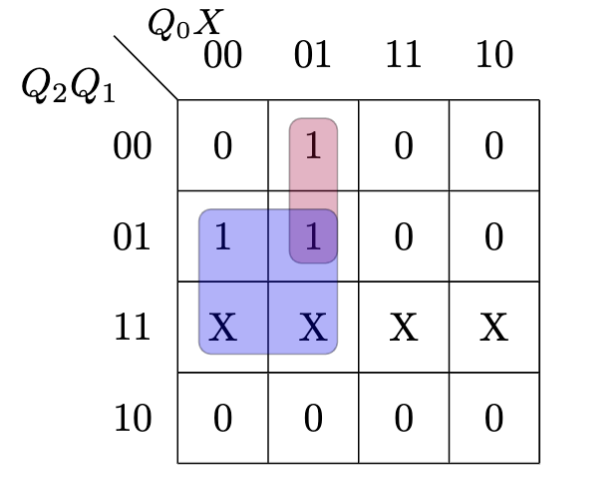
\includegraphics[width=0.6\textwidth]{/y.png}
      \caption{K-Map for $Output\ (Y)$}
  \end{minipage}
  \begin{minipage}[c]{0.45\textwidth}
      \centering
      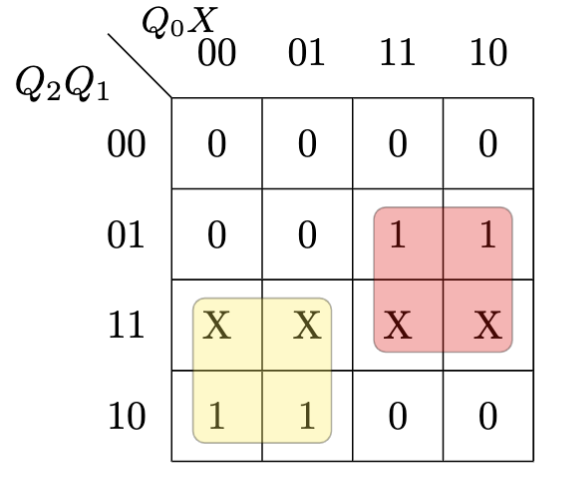
\includegraphics[width=0.6\textwidth]{/d2.png}
      \caption{K-Map for $D_{2}$}
  \end{minipage}
\end{figure}
\begin{figure}[H]
  \centering
  \begin{minipage}[c]{0.45\textwidth}
    \centering
    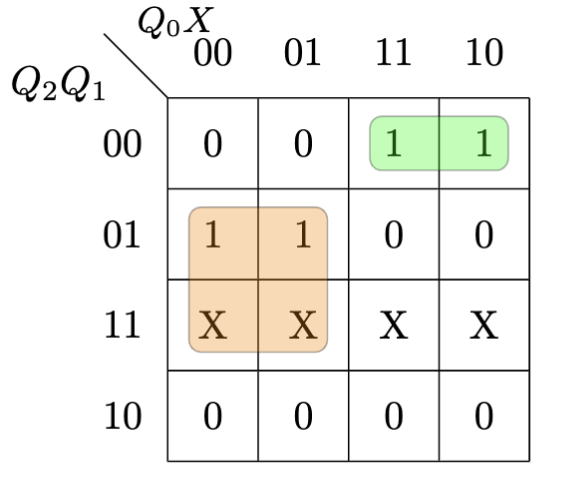
\includegraphics[width=0.6\textwidth]{/d1.png}
    \caption{K-Map for $D_{1}$}
\end{minipage}
  \begin{minipage}[c]{0.45\textwidth}
      \centering
      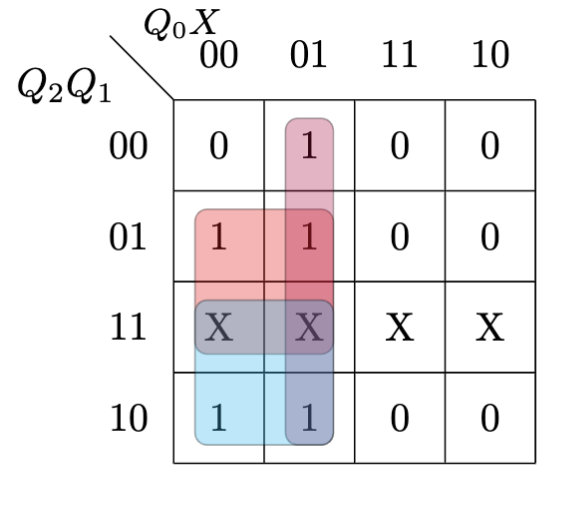
\includegraphics[width=0.6\textwidth]{/d0.png}
      \caption{K-Map for $D_{0}$}
  \end{minipage}
\end{figure}
And from the k-maps the simplified expressions are as follows:
$$ Y = \bar{Q_{2}}\bar{Q_{0}}X \ +\  Q_{1}\bar{Q_{0}}$$
$$ D_{2} = Q_{2}\bar{Q_{0}}\ +\ Q_{0}Q_{1}$$
$$ D_{1} = \bar{Q_{2}}\bar{Q_{1}}Q_{0}\ +\ Q_{1}\bar{Q_{0}}$$
$$ D_{0} = \bar{Q_{0}}X\ +\ Q_{1}\bar{Q_{0}}\ +\ Q_{2}\bar{Q_{0}}$$
\section{Verilog Simulation}
\subsection{Code}
The code file (design.v) for the implementation of the above finite state machine using D-flipflops is:
The D-flipflop designed is a postive edge triggered one and has a reset pin which is active low.
\inputminted[bgcolor=bg,frame=lines,framesep=2mm,numbers=left]
{Verilog}{./code-files/design.v}

The code file for the testbench (main.v) is:
Intitially the input (X) is kept 1 for atleast 6 clock cycles and when it reaches the idle state again, it is then made 0 for again atleast 6 clock cycles, and finally it is again made 1 for one clock cycle so that machine again becomes active then immediately made 0 for again atleast 6 clock cycles.
The D-flipflop designed is a postive edge triggered one and has a reset pin which is active low.
\inputminted[bgcolor=bg,frame=lines,framesep=2mm,numbers=left]
{Verilog}{./code-files/main.v}
\subsection{Waveform}
The gtkwave plot obtained is:
\begin{figure}[H]
  \centering
  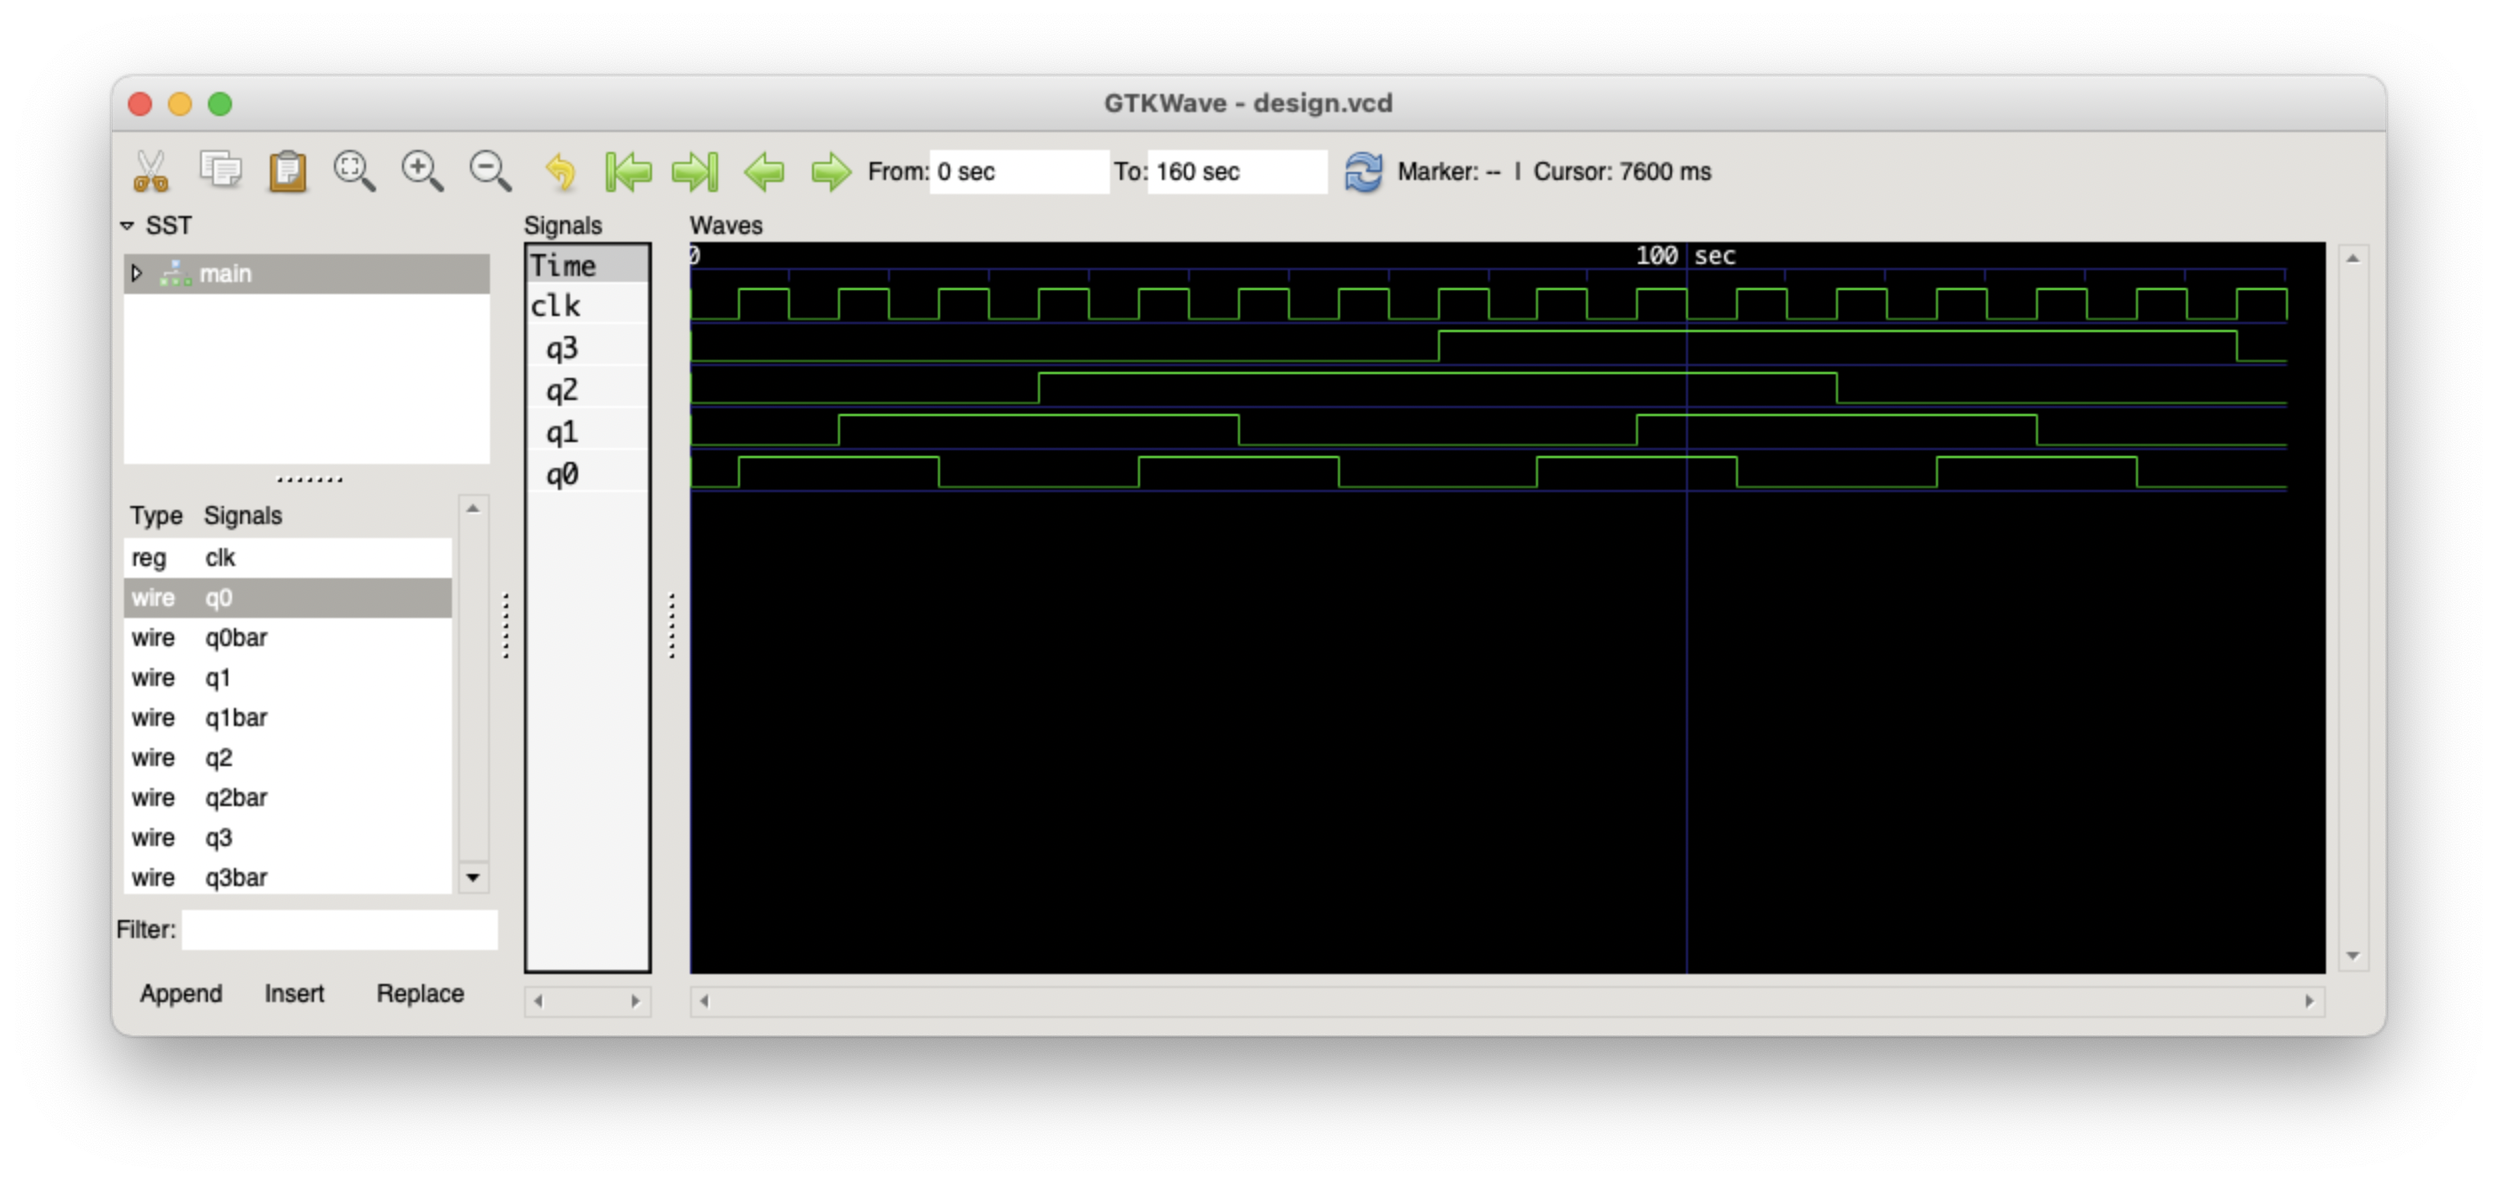
\includegraphics[width=1.1\textwidth]{/plot.png}
\end{figure}
Hence it can be observed from the plot, that the FSM once starts generating the sequence, keep generating it no matter whatever is the value of X is and also it remains in the idle state as long as X is kept 0. And at last the sequence generated is $1,0,1,0,0,0$ at the output side. Hence, the FSM is working perfectly as required.
\section*{Download link for the code files}
The code files can be downloaded from \href{https://drive.google.com/file/d/154Ns-3BjkBaJXzXriUoTww2TzG_f4Ziu/view?usp=sharing}{\textbf{here}}.


\end{document}

% \begin{tikzpicture}
%   \node[state,line width=0.3mm] (s0) at (0,0) {$S_{0}$} ;
%   \node[state,line width=0.3mm] (s1) at (3.5,0) {$S_{1}$} ;
%   \node[state,line width=0.3mm] (s2) at (7,0) {$S_{2}$} ;
%   \node[state,line width=0.3mm] (s3) at (7,-2.5) {$S_{3}$} ;
%   \node[state,line width=0.3mm] (s4) at (3.5,-2.5) {$S_{4}$} ;
%   \node[state,line width=0.3mm] (s5) at (0,-2.5) {$S_{5}$} ;
%   \draw[->,line width=0.3mm] (s0) edge [loop above] node[above]{$0/0$} (s0);
%   \draw[-stealth,line width=0.3mm] (s0) edge [bend left,above] node {$1/1$} (s1);
%   \draw[-stealth,line width=0.3mm] (s1) edge [bend left,above] node {$0/0$} (s2);
%   \draw[-stealth,line width=0.3mm] (s1) edge [bend right,below] node {$1/0$} (s2);
%   \draw[-stealth,line width=0.3mm] (s2) edge [bend left,right] node {$1/1$} (s3);
%   \draw[-stealth,line width=0.3mm] (s2) edge [bend right,left] node {$0/1$} (s3);
%   \draw[-stealth,line width=0.3mm] (s3) edge [bend left,below] node {$0/0$} (s4);
%   \draw[-stealth,line width=0.3mm] (s3) edge [bend right,above] node {$1/0$} (s4);
%   \draw[-stealth,line width=0.3mm] (s4) edge [bend left,below] node {$0/0$} (s5);
%   \draw[-stealth,line width=0.3mm] (s4) edge [bend right,above] node {$1/0$} (s5);
%   \draw[-stealth,line width=0.3mm] (s5) edge [bend left,left] node {$1/0$} (s0);
%   \draw[-stealth,line width=0.3mm] (s5) edge [bend right,right] node {$0/0$} (s0);
% \end{tikzpicture}

% \begin{circuitikz}
%   \ctikzset{logic ports=ieee}
%   \ctikzset{logic ports/fill=mygray}
%   \ctikzset{multipoles/flipflop/clock wedge size=0.3}
%   \node (clk) at (-4,-2){\textbf{Clk}};
%   \node (x) at (-4,2){\textbf{X}};
%   \node (x1) at (-4,2.5){$Q_{2}$};
%   \node (x2) at (-4,3){$Q_{1}$};
%   \node (x3) at (-4,3.5){$Q_{0}$};
%   \node (x4) at (-4,-2.5){$\bar{Q_{2}}$};
%   \node (x5) at (-4,-3){$\bar{Q_{1}}$};
%   \node (x6) at (-4,-3.5){$\bar{Q_{0}}$};

%   \node [flipflop D,
%       flipflop def={t1=$D_{2}$,t6=$Q_{2}$,t4=\ctikztextnot{$Q_{2}$},c3=1},fill=mygray
%   ](d1) at (-1,0){};
%   \node [flipflop D,
%       flipflop def={t1=$D_{1}$,t6=$Q_{1}$,t4=\ctikztextnot{$Q_{1}$},c3=1},fill=mygray
%   ](d2) at (4,0){};
%   \node [flipflop D,
%       flipflop def={t1=$D_{0}$,t6=$Q_{0}$,t4=\ctikztextnot{$Q_{0}$},c3=1},fill=mygray
%   ](d3) at (9,0){};

%   \draw (x1) -- (11,2.5);
%   \draw (x2) -- (11,3);
%   \draw (x3) -- (11,3.5);
%   \draw (x) -- (11,2);
%   \draw (clk) -- (11,-2);
%   \draw (x4) -- (11,-2.5);
%   \draw (x5) -- (11,-3);
%   \draw (x6) -- (11,-3.5);

%   \node (clk1) at ($(d1.pin 3)+(-0.1,0)$){};
%   \draw (d1.pin 3) node[branch]{} -| (clk1 |- clk) node[branch]{};
%   \node (clk2) at ($(d2.pin 3)+(-0.1,0)$){};
%   \draw (d2.pin 3) node[branch]{} -| (clk2 |- clk) node[branch]{};
%   \node (clk3) at ($(d3.pin 3)+(-0.1,0)$){};
%   \draw (d3.pin 3) node[branch]{} -| (clk3 |- clk) node[branch]{};

%   \draw (d1.pin 6)node[branch]{} -- (d1.pin 6 |- x1) node[currarrow,rotate=90]{};
%   \draw (d2.pin 6)node[branch]{} -- (d2.pin 6 |- x2) node[currarrow,rotate=90]{};
%   \draw (d3.pin 6)node[branch]{} -- (d3.pin 6 |- x3) node[currarrow,rotate=90]{};
%   \draw (d1.pin 4)node[branch]{} -- (d1.pin 4 |- x4) node[currarrow,rotate=-90]{};
%   \draw (d2.pin 4)node[branch]{} -- (d2.pin 4 |- x5) node[currarrow,rotate=-90]{};
%   \draw (d3.pin 4)node[branch]{} -- (d3.pin 4 |- x6) node[currarrow,rotate=-90]{};

%   \ctikzset{logic ports/scale=0.5}
%   \node[or port,draw] at ($(d1.pin 1)+(-1,0)$) (xor1) {};

% \end{circuitikz}